\chapter{Analysis and Design Approach} \label{chapter:analysis_and_design}
\section{Previous Architecture}
The previous architecture of the ASR system, as illustrated in Figure \ref{fig:previous_architecture}, was deployed on a Kubernetes cluster hosted on AWS.

Transcription requests were routed through an NGINX Ingress Controller, which forwarded them to a master pod responsible for managing transcription tasks. Upon receiving a request, the master pod authenticated it and, if a worker pod was available, initiated a WebSocket connection. The audio data was then forwarded to a worker pod for transcription.

Each worker pod was associated with a model attached via a Persistent Volume Claim (PVC). After processing, the worker pod sent the transcription results back to the master pod, which then forwarded them to the client.

\section{Challenges and Design Evolution}
Based on the evaluation of the previous architecture in Section \ref{section:challenges}, several challenges were identified. The new design addresses these by adopting a more decoupled, scalable, and fault-tolerant approach.

\subsection{Decoupling Master and Worker Pods}
The reliance on synchronous WebSocket communication between the master and worker pods introduced significant challenges in fault tolerance and scaling. Any failure in either component would disrupt ongoing transcription tasks. Additionally, scaling worker pods dynamically was constrained by the direct communication with the master pod.

\subsubsection{Proposed Solution: Asynchronous Messaging}
To enhance scalability and resilience, the new architecture adopts a message queue approach using RabbitMQ (Figure \ref{fig:decouple}).
\begin{figure}[!ht]
    \centering
    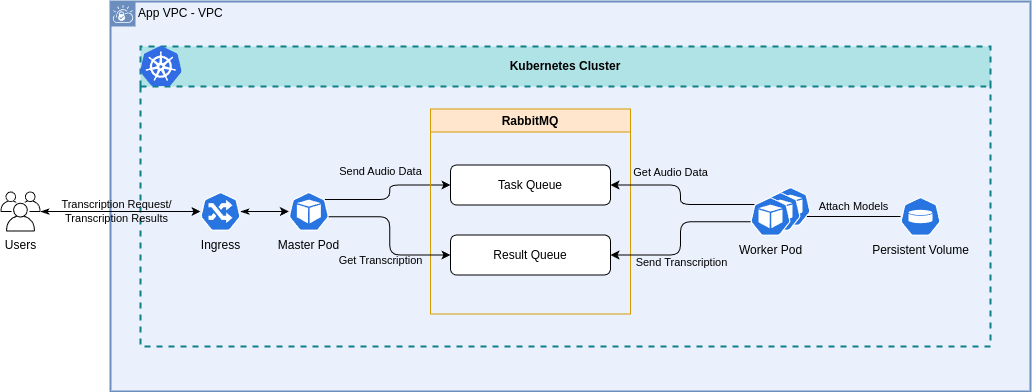
\includegraphics[width=\textwidth]{figures/decouple.drawio.png}
    \caption{Decoupling the Master and Worker Pods}
    \label{fig:decouple}
\end{figure}

In the new design, the master pod publishes transcription tasks to a RabbitMQ task queue. Worker pods asynchronously consume tasks, process the audio, and publish results to a results queue. The master pod retrieves transcription results and sends them back to the client. This design eliminates direct dependencies between components, allowing independent scaling and improved fault tolerance.

\subsection{Enhancing State Management and Fault Tolerance}
Previously, the worker pods stored audio data in an in-memory queue. If a worker pod crashed, all buffered data would be lost, requiring clients to retransmit. This dependency on volatile storage complicated recovery and degraded system reliability.

\subsubsection{Proposed Solution: Redis for State Persistence}
To mitigate data loss and improve fault tolerance, the application state is now stored in Redis, ensuring that if a service fails, it can recover essential state information. Additionally, RabbitMQ’s message durability ensures that queued transcription tasks are not lost if a worker crashes. If a worker pod fails mid-transcription, a new worker can pick up the task from the queue without requiring client intervention. This redesign significantly enhances fault tolerance and ensures a seamless recovery mechanism.

\subsection{Scaling and Load Management}
The previous deployment relied on a single master pod, creating a single point of failure. Additionally, worker scaling required manual interventions, making it inefficient and slow in responding to traffic fluctuations.

\subsubsection{Proposed Solution: Kubernetes Autoscaling and Worker Manager}
The new architecture incorporates:
\begin{itemize}
    \item \textbf{Kubernetes Horizontal Pod Autoscaler (HPA):} Automatically scales master pods based on request load, preventing service disruptions.
    \item \textbf{Dynamic Worker Scaling via Worker Manager:} A new Worker Manager service dynamically adjusts worker pod replicas based on configurable \texttt{SCALING\_TARGET} (See Code \ref{lst:worker_scaling}).
\end{itemize}

The dynamic scaling policy is managed by an additional service called the Worker Manager, which is described in detail in \hyperref[section:worker_manager]{\textit{Chapter 4: Detailed Implementation}}. The Worker Manager monitors the current state of worker pods for each model and adjusts the number of pods accordingly to maintain the scaling target.

Key features of this solution include:
\begin{itemize}
    \item \textbf{Load-based scaling:}  The Worker Manager scales worker pods up or down based on current traffic and processing load, ensuring optimal resource utilization.
    \item \textbf{Minimized scaling disruptions:}  To prevent excessive scaling activity, the scaling policy incorporates a configurable \texttt{CHECK\_INTERVAL} that limits the frequency of scaling operations.
\end{itemize}

\subsection{Improving Documentation and Code Readability}
The previous ASR system codebase lacked sufficient documentation, making it difficult to onboard new developers and troubleshoot issues. Without clear documentation, understanding system behavior and implementing new features were time-consuming.

\subsubsection{Proposed Solution: Structured Documentation Strategy}
To address these challenges, the new codebase will prioritize comprehensive and clear documentation. A detailed \texttt{README} file will provide an overview of the project, including its architecture, purpose, and key components. Additionally, inline comments will be incorporated throughout the codebase to explain the functionality and intent of each component.

This documentation strategy offers two key benefits:
\begin{enumerate}
    \item \textbf{Faster Developer Onboarding:} New developers can quickly grasp system functionalities with clear explanations and structured guidance.
    \item \textbf{Improved Maintainability:} Well-documented code ensures future modifications can be made efficiently without extensive reverse engineering.
\end{enumerate}

Even a simple inline comment describing a function’s purpose and parameters can significantly improve readability. For instance, Code \ref{lst:code_documentation} demonstrates how a well-placed comment enhances code clarity.

By integrating structured documentation and inline comments into the development workflow, the new codebase will be easier to maintain and scale, reducing onboarding time and improving long-term sustainability.
